\section{Heimspeicher}

\subsection{Alternative Speichernutzung für Heimspeicher}

\begin{itemize}
    \item Bezugsleistung begrenzen (Peak-Shaving)
    \begin{itemize}
        \item Einhalten der Maximalleistung des Netzanschlusses (z.B. E-Mobilität)
        \item Senkung der Stromkosten bei Leistungspreisen
    \end{itemize}

    \item Einspeiseleistung begrenzen
    \begin{itemize}
        \item Lokal: Netzausbau vermeiden (x kWp am Netzverknüpfungspunkt möglich)
        \item Überregional, längerfristig: PV-Überschüsse vermeiden
    \end{itemize}

    \item Ausnutzung von Tarifunterschieden (Arbitrage)
    \begin{itemize}
        \item Lastverschiebung in Niedertarifzeiten (Doppeltarif, flexible Stromtarife)
    \end{itemize}

    \item Schwarmspeicher (Pooling)
    \begin{itemize}
        \item Regelleistung (primär, sekundär)
    \end{itemize}

    \item Speicherstrategien zur Verlängerung der Lebensdauer
\end{itemize}


\subsection{Reduktion von Netzbezugsleistung}

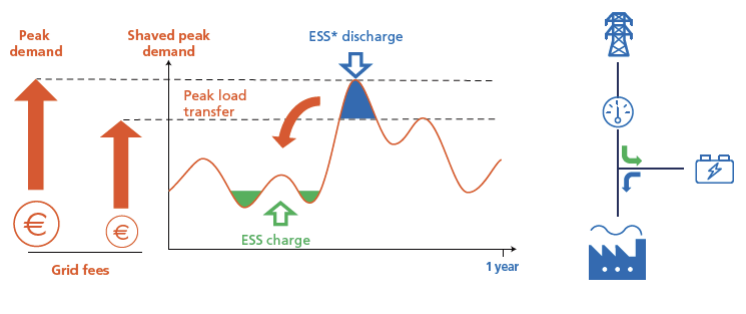
\includegraphics[width=0.98\linewidth]{images/Reduktion_Netzbezugsleistung.png}

\begin{itemize}
    \item Minimieren der monatlichen Leistungsspitze
    \begin{itemize}
        \item Reduziert die Kosten für größere Verbraucher mit Leistungstarif
    \end{itemize}
\end{itemize}



\subsubsection{... durch Wärmepumpe und Betterie}

\begin{itemize}
    \item Jahresdauerlinie Netzbezug
    \begin{itemize}
      \item PV-Leistung 7{,}2 kWp, Stromverbrauch ca. 7'200 kWh/a
      \item Mit einer 6 kWh / 6 kW Batterie können die Netzbezugsspitzen deutlich reduziert werden
    \end{itemize}
\end{itemize}

\vspace{0.15cm}

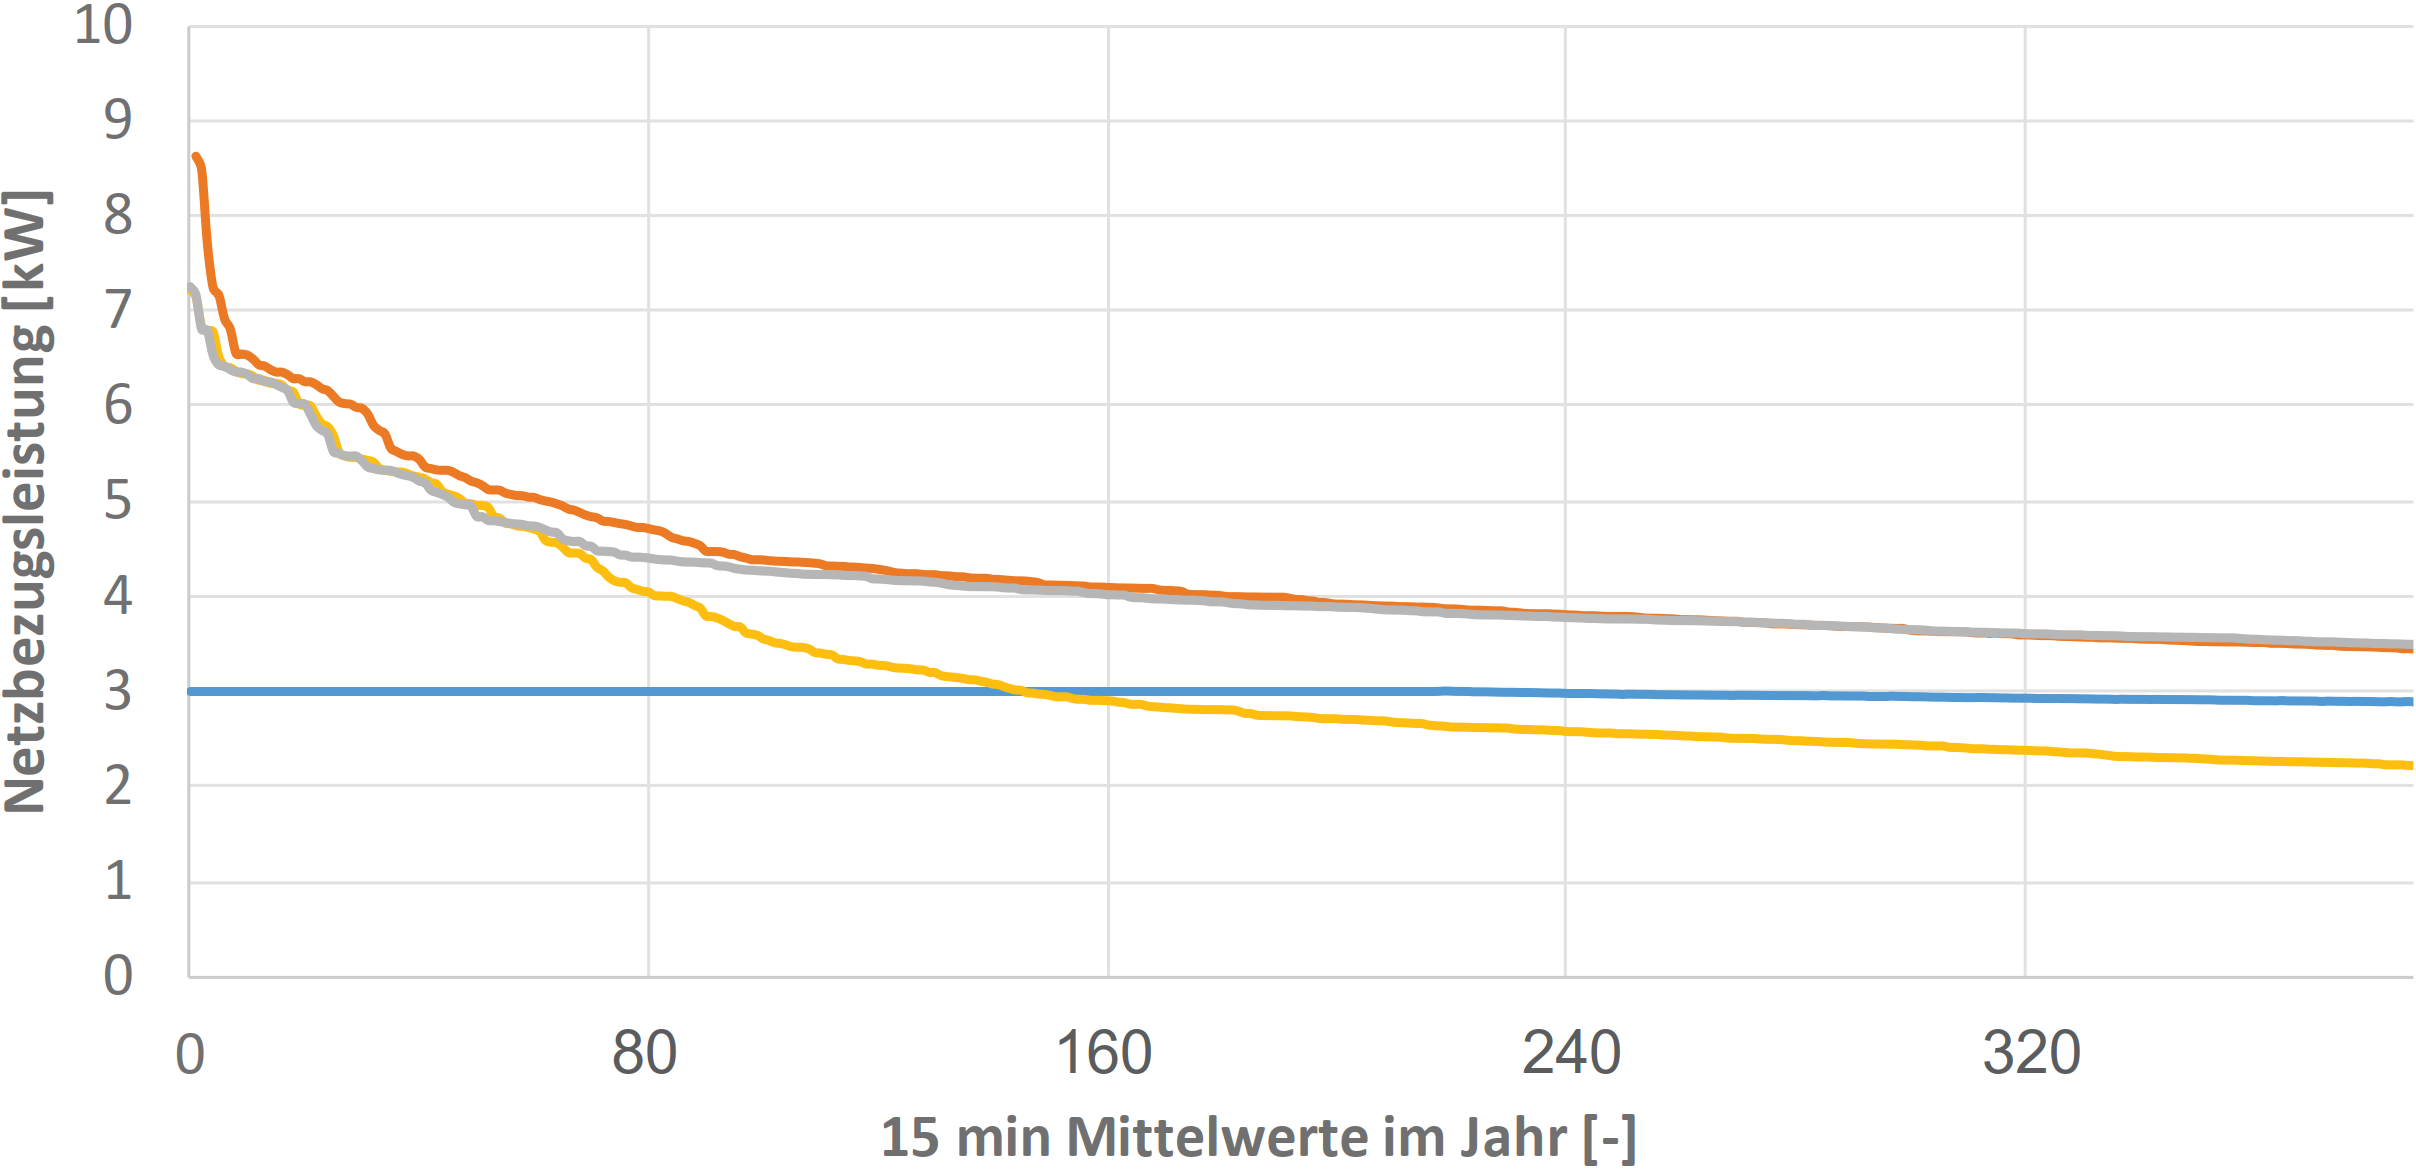
\includegraphics[width=0.98\linewidth]{images/Durch_Wärmepumpen_und_Batterien_1.png}

\vspace{0.15cm}

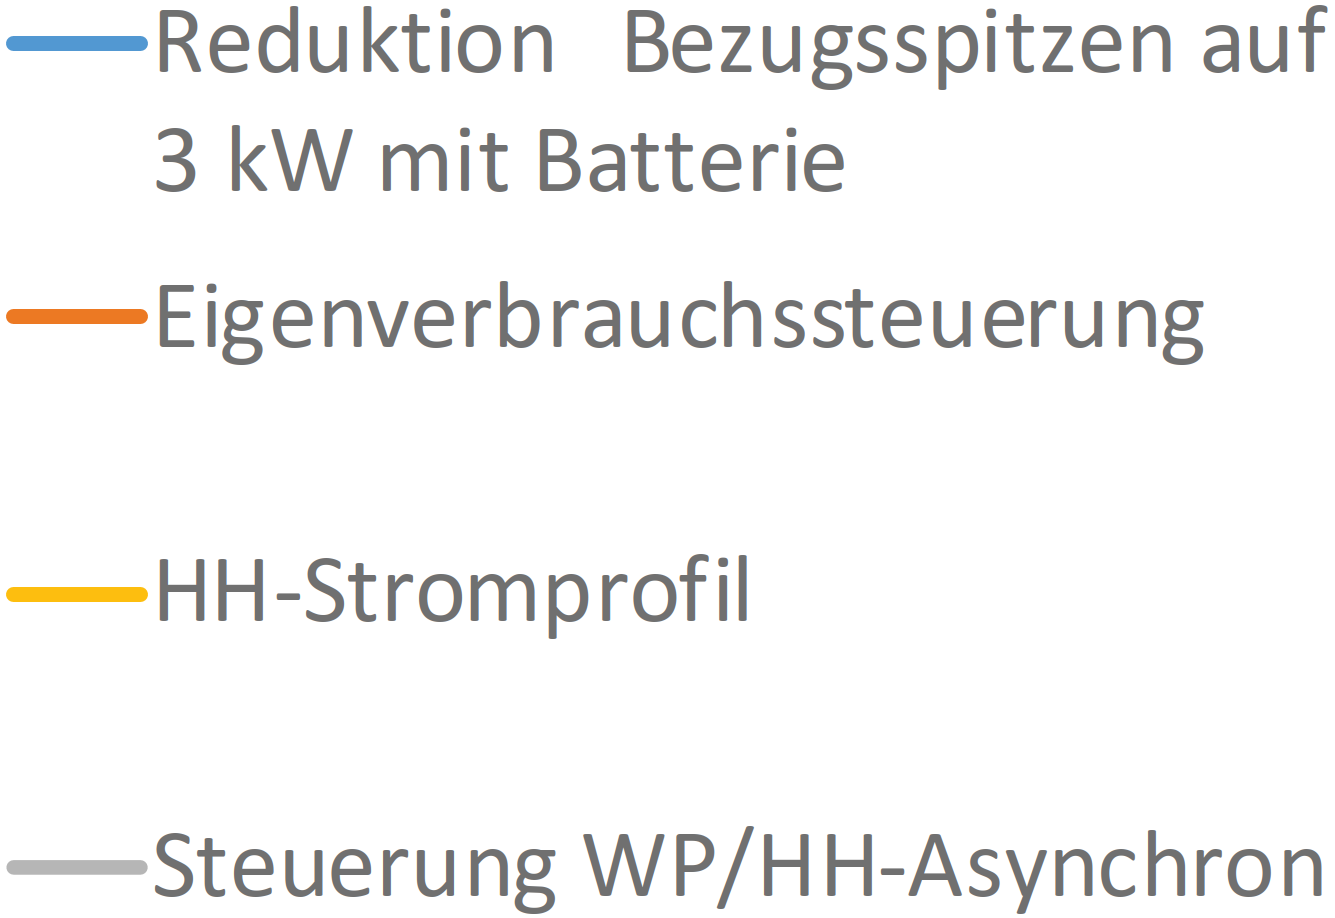
\includegraphics[width=0.35\linewidth]{images/Durch_Wärmepumpen_und_Batterien_2.png}



\subsection{Reduktion von Einspeiseleistung}

\subsubsection{Konventionelle Speicherung}
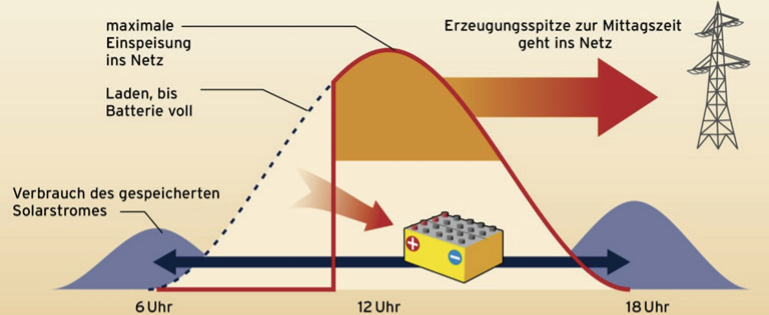
\includegraphics[width=0.98\linewidth]{images/Konventionelle_Speicherung.png}

\subsubsection{Netzoptimierte Speicherung}
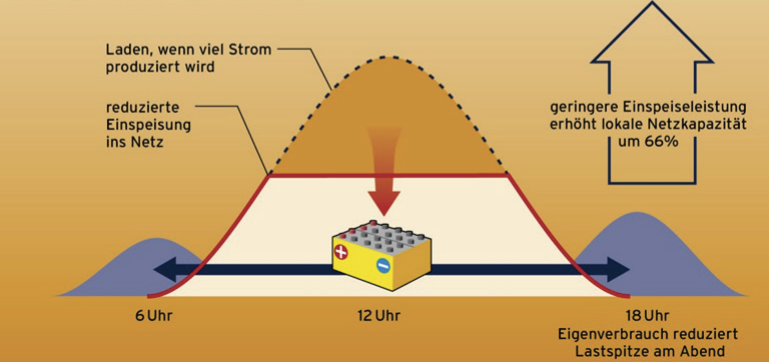
\includegraphics[width=0.98\linewidth]{images/Netzoptimierte_Speicherung.png}



\subsection{Reduktion der Netzeinspeiseleistung}

\begin{itemize}
    \item Verschiedene Betriebsstrategien
    \begin{itemize}
      \item Jahresmittlerer Tagesgang der Einspeiseleistung (links) und Jahresdauerlinien der Einspeiseleistung (rechts)
      \item PV-Leistung 5 kWp, nutzbare Speicherkapazität 5 kWh
    \end{itemize}
\end{itemize}

\vspace{0.15cm}

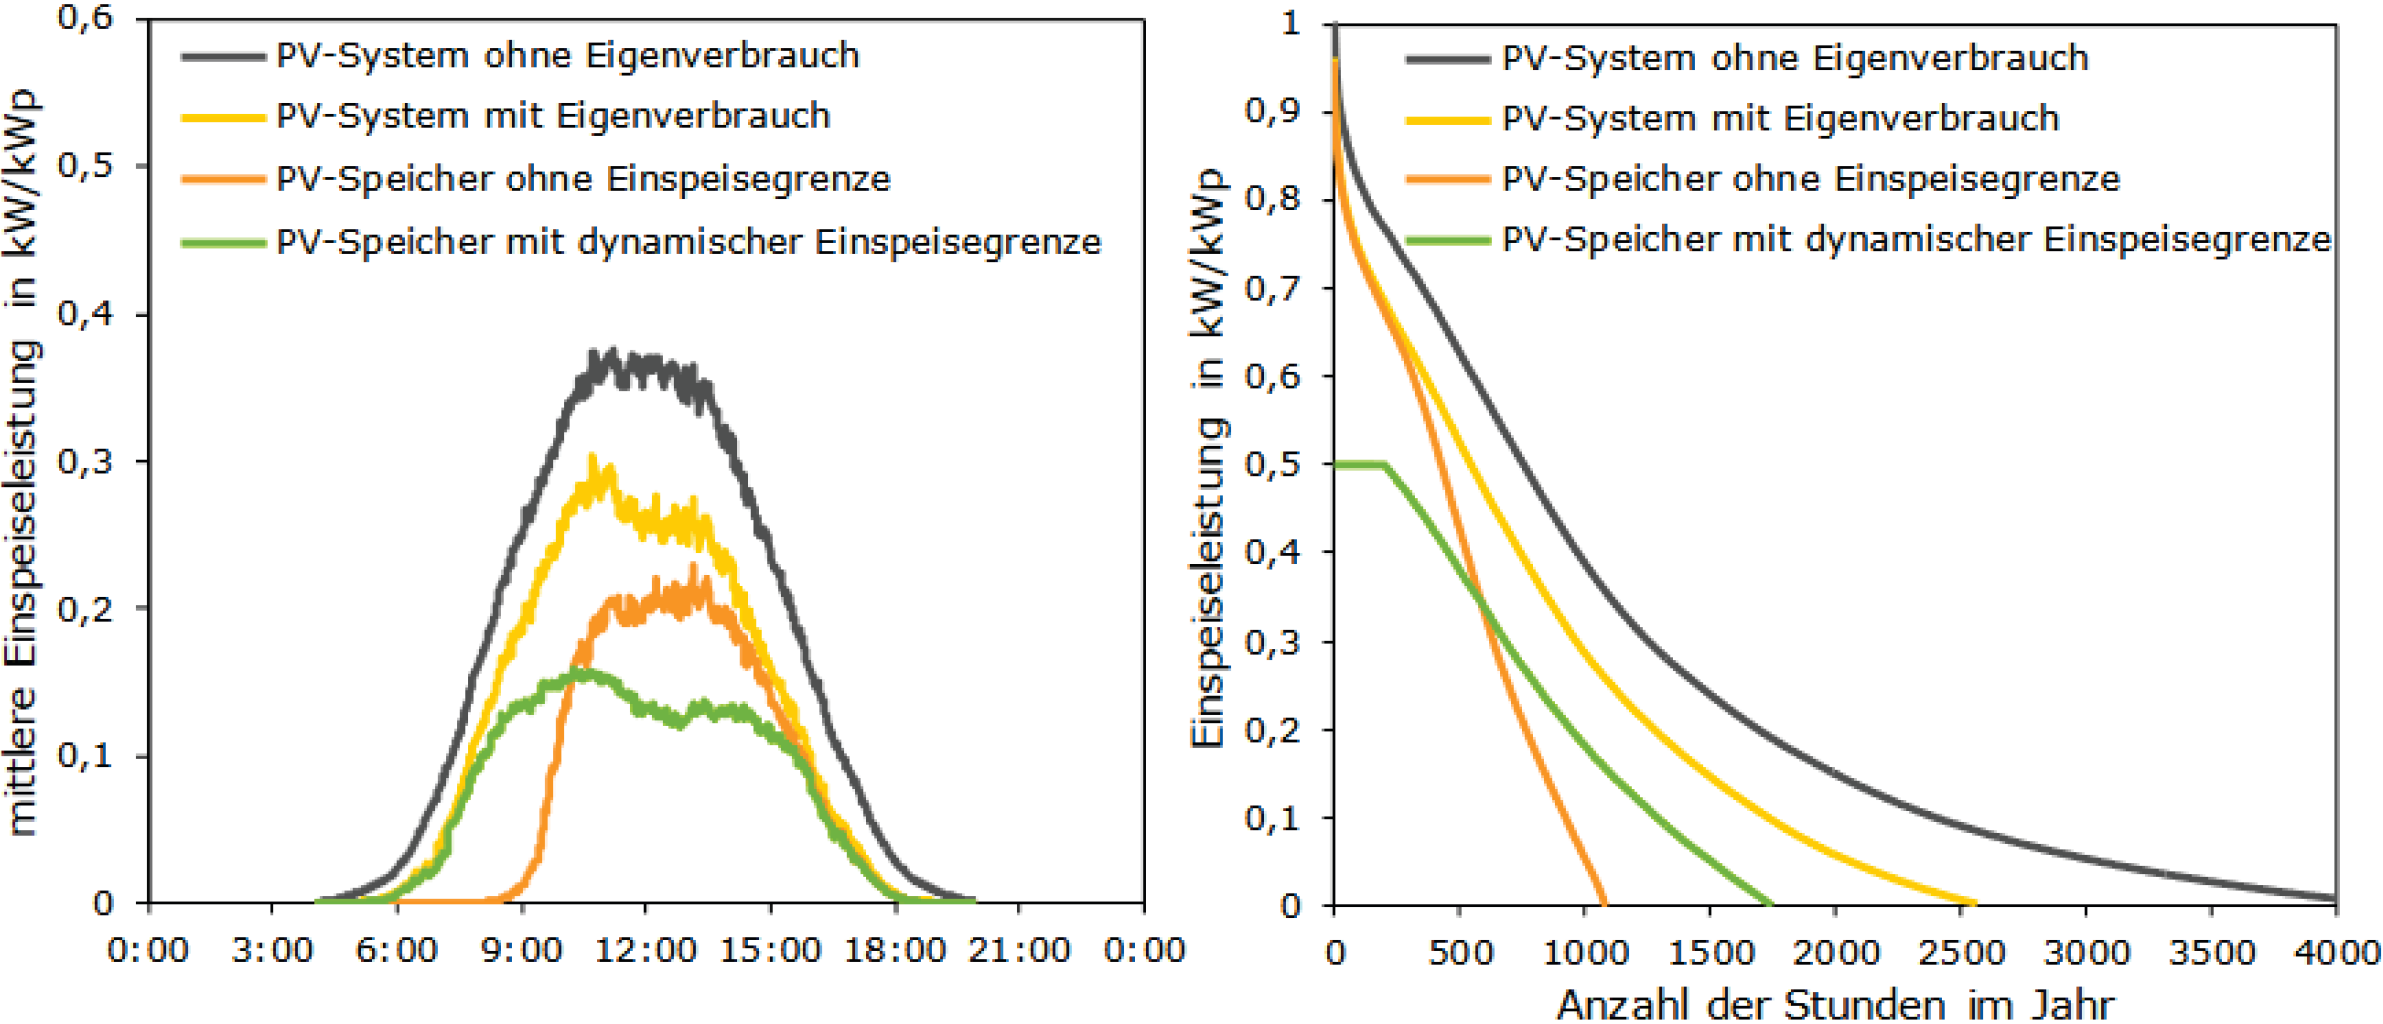
\includegraphics[width=0.98\linewidth]{images/Reduktion_der_Netzeinspeiseleistung.png}

\subsubsection{Beispiel mit 8 kWp}
\begin{itemize}
    \item Begrenzung der Einspeiseleistung am Netzverknüpfungspunkt auf 
    50 \% der nominalen PV-Generatorleistung (4 kWp)
\end{itemize}

\begin{minipage}[c]{0.49\columnwidth}
    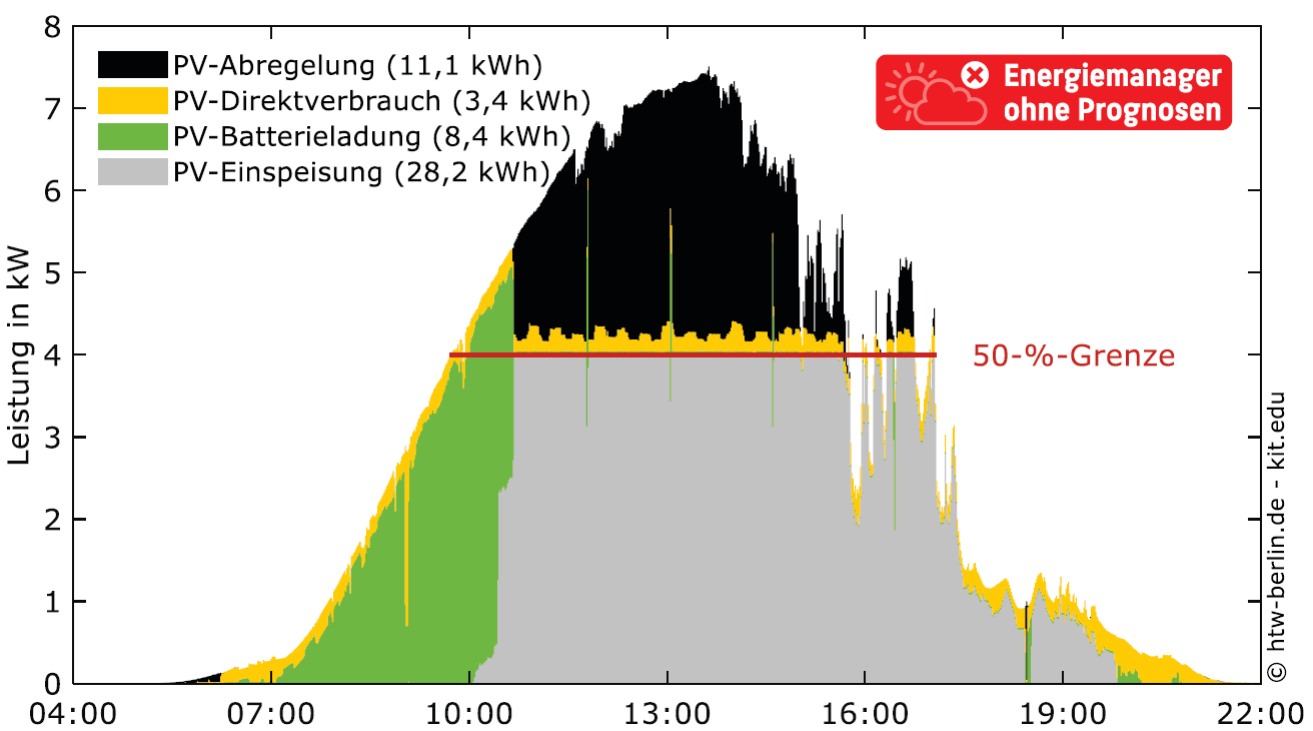
\includegraphics[width=0.98\columnwidth]{images/Reduktion_der_Netzeinspeiseleistung_Beispiel_1.png}
\end{minipage}
\hfill
\begin{minipage}[c]{0.49\columnwidth}
    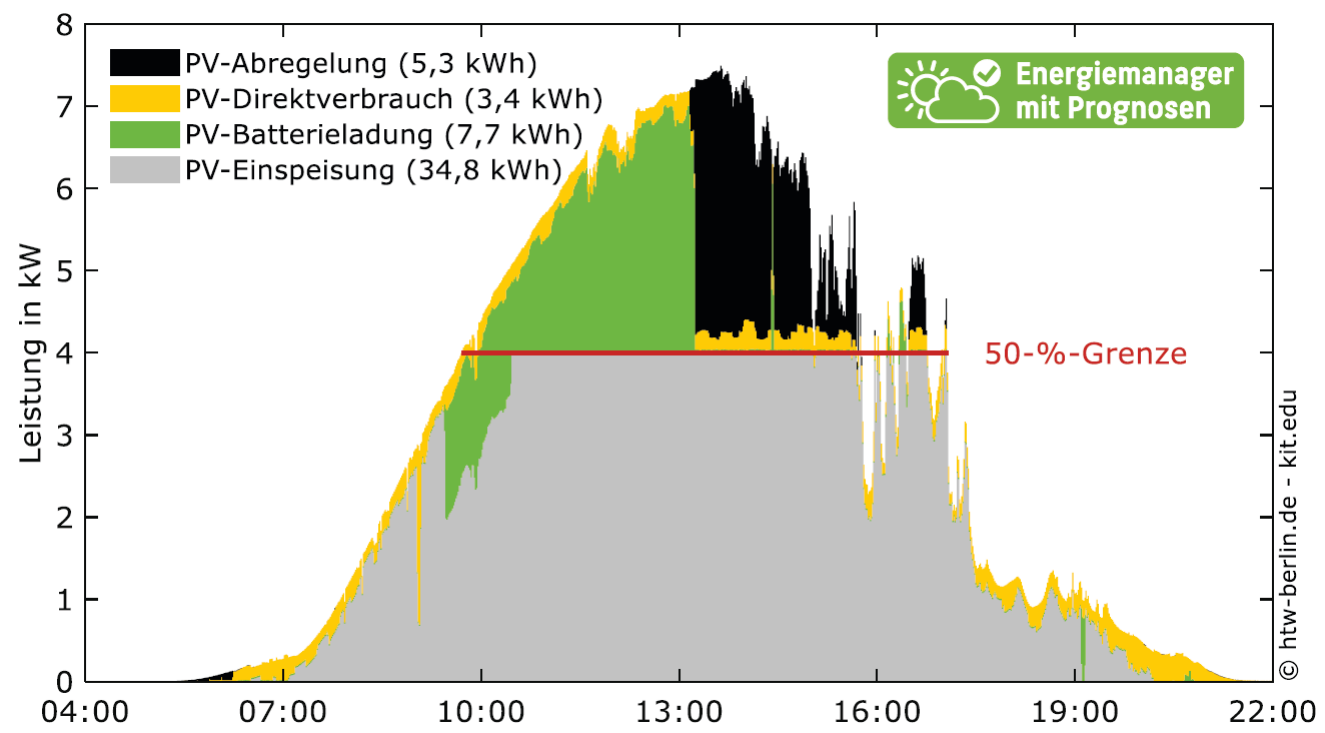
\includegraphics[width=0.98\columnwidth]{images/Reduktion_der_Netzeinspeiseleistung_Beispiel_2.png}
\end{minipage}


\subsubsection{Abregelungsverluste}

Die resultierende Höhe der \textbf{Abregelungsverluste} hängt unter anderem von folgender Eigenschaften der PV-Speichersysteme ab:
\begin{itemize}
  \item Nutzbare Speicherkapazität des Batteriespeichers
  \item Nennleistung des Wechselrichters und des Batteriespeichers
  \item Wechselrichter- und Batteriewirkungsgrad
  \item Güte der Prognosen (PV-Leistung und elektrische Last)
  \item Güte der Ladezustandsbestimmung
  \item Qualität des Optimierungsalgorithmus
  \item Qualität der Regelung zum schnellen Ausgleich von Prognosefehlern
  \item Dauer bis zur nächsten Aktualisierung des Ladefahrplans
  \item Abregelungsverhalten (Möglichkeit der stufenlosen Abregelung)
\end{itemize}


\subsubsection{Prognosebasierte Steuerung mit selbstlernendem Algorithmus}

\begin{tabular}{|l|c|c|c|}
    \hline
     & S1 & S2 & S3\\
    \hline
    DC-Zykleneffizienz & 91{,}5\,\% & 92{,}1\,\% & 92{,}6\,\% \\
    \hline
    Gesamtsystemeffizienz & 91{,}7\,\% & 90{,}4\,\% & 88{,}6\,\% \\
    \hline
    Autarkiegrad & 47{,}4\,\% & 47{,}8\,\% & 47{,}4\,\% \\
    \hline
\end{tabular}

\vspace{0.15cm}

S1: Normale Steuerung\\
S2: Leistungsreduzierung auf 70\,\%\\
S3: Leistungsreduzierung auf 50\,\%

\subsection{Betriebsstrategien zur Verlängerung der Lebensdauer}

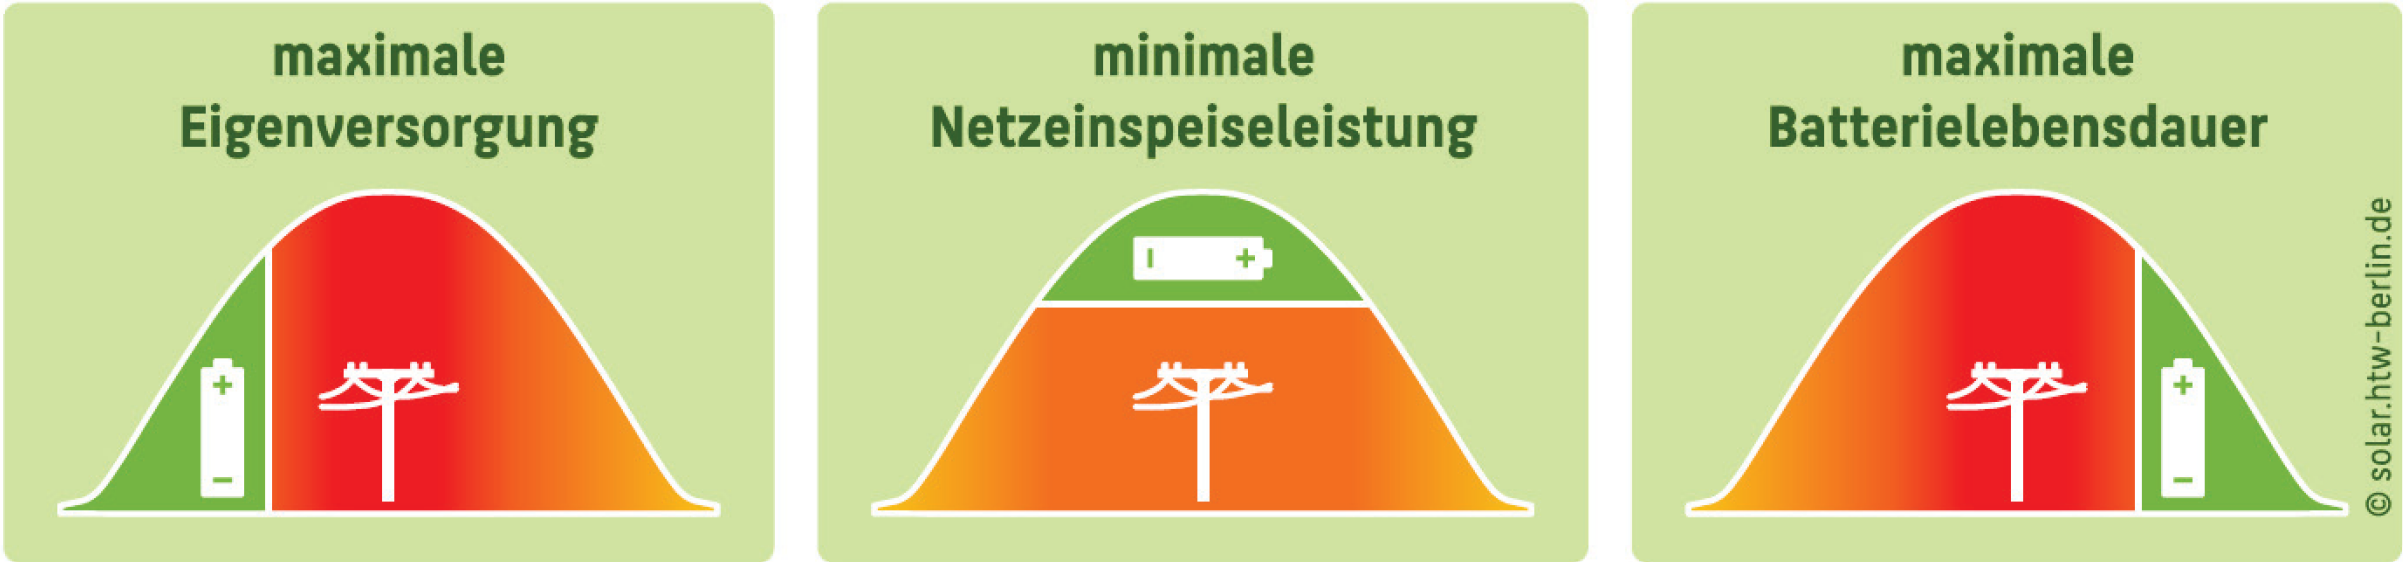
\includegraphics[width=0.98\columnwidth]{images/Betriebsstrategie_zur_Verlängerung_der_Lebensdauer.png}

\vspace{0.15cm}

\begin{tabular}{@{}lll@{}}
\toprule
\textbf{Ladestrategie} & \textbf{Zeitpunkt}       & \textbf{Standzeit $>$ 90\,\% Ladezustand} \\ \midrule
Frühzeitig              & Vormittags                  & 99\,h                                     \\
Prognosebasiert         & Mittags                  & 72\,h                                     \\
Prognosebasiert         & Nachmittags              & 43\,h                                     \\ \bottomrule
\end{tabular}

\textbf{Hinweis:} Je kürzer die Lithium-Batterie vollständig geladen ist, desto langsamer altert sie.




\subsection{Elektromobilität als Heimspeicher}
\begin{itemize}
    \item Als Verbraucher / steuerbare Last
    \begin{itemize}
      \item Integration ins Lastmanagement / Energiemanagementsystem (EMS)
    \end{itemize}
    \item Als Stromspeicher
    \begin{itemize}
      \item Bidirektionales Laden / Vehicle-to-Home (V2H)
    \end{itemize}
  \end{itemize}
























